\subsection{Baseline model} \label{baseline_model}
The architecture of the baseline network used in the experiments is shown in Figure~\ref{fig:et_baseline_architecture}. Starting from the input, the text is composed of three parts: left context (LC), mention (M), and right context (RC). The encoder receives a sequence in the form of \verb|[CLS]M[SEP]LC[SEP]RC|.  The example in the picture reports BERT as encoder, but any variant could be used to take its place. The versions used to perform the experiments of this thesis are BERT large\footnote{https://huggingface.co/bert-large-cased} and DistilBERT\footnote{https://huggingface.co/distilbert-base-uncased} for PyTorch\footnote{https://pytorch.org/}. In any case, the encoders are trained using the adapters with the Pfeiffer strategy. The framework used to integrate them into the models is AdapterHub\footnote{https://github.com/Adapter-Hub/adapter-transformers}. Once the encoder produces the output sequence, the encoding of the \verb|[CLS]| token is fed into a basic neural network composed of a fully connected layer and a classification layer. The fully connected layer has the same dimension as the encoder's output, the classification layer applies the sigmoid activation function to compute the probability to assign each label. Finally, there is the inference step to obtain the final predictions starting from the probabilities (more details in section~\ref{inference_rules}).

\begin{figure}[H]
    \centering
    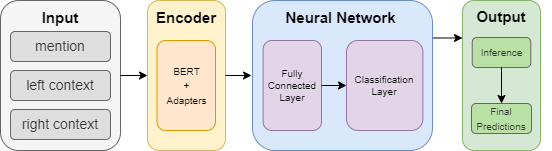
\includegraphics[width=.8\linewidth]{figures/et_baseline_architecture.png}
    \caption{Baseline model architecture}
    \label{fig:et_baseline_architecture}
\end{figure}


\subsection{KENN model} \label{kenn_model}
The architecture of the KENN-based model is designed starting from the baseline. As we can see in Figure~\ref{fig:et_kenn_architecture}, the architecture of the two models is almost the same. The only differences are the presence of KENN in the middle of the network and the KB provided to the model. The knowledge enhancement layer is placed between the fully connected layer and the classification layer. What said for the baseline model about input representation, encoders, etc. is still valid for this model.

\begin{figure}[H]
    \centering
    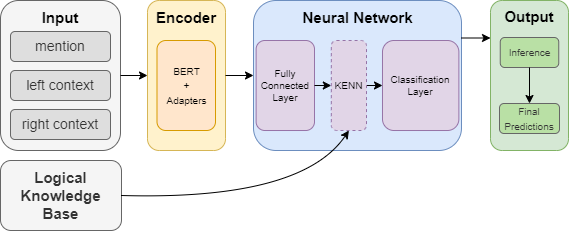
\includegraphics[width=.8\linewidth]{figures/et_kenn_architecture.png}
    \caption{KENN-based model architecture}
    \label{fig:et_kenn_architecture}
\end{figure}

Among the strategies for defining logical KB proposed in section~\ref{knowledge_generation}, the ones chosen for the experiments are the \textit{Bottom Up}, \textit{Top Down}, and \textit{Hybrid}. Other KB modes from Table~\ref{tab:kb_modes} are not taken into account since they do not apply to datasets with a 2-level hierarchy. We will not even analyze horizontal constraints since the priority has been given to the vertical ones. The number of clauses generated by the chosen KB modes are reported in Table~\ref{tab:dataset_clauses}.

\begin{table}
\centering
\caption{Datasets and number of clauses}
\label{tab:dataset_clauses}
\begin{tabular}{|c|ccc|}
\hline
\textbf{Dataset} & \multicolumn{1}{c|}{\textbf{Bottom Up}} & \multicolumn{1}{c|}{\textbf{Top Down}} & \textbf{Hybrid} \\ \hline
BBN              & 31                                      & 9                                      & 40              \\ \hline
FIGER            & 79                                      & 22                                     & 101             \\ \hline
\end{tabular}
\end{table}

Depending on the KB mode, KENN affects the predictions of the baseline network in different ways. Some statistics about the influence of the logical knowledge are available in Table~\ref{tab:dataset_stats_kenn}, which provides the following information:
\begin{itemize}
    \item \textbf{\% no clauses:} percentage of examples labeled with at least one type that does not occur in any clause (i.e. isolated type)
    \item \textbf{\% no clauses (strict):} percentage of examples labeled exclusively with types that do not occur in any clause (i.e. isolated types only)
    \item \textbf{\% inappropriate Top Down rules:} percentage of examples in which a supertype occurs without any of its subtypes; equivalent to \textit{\% only supertype} in Table~\ref{tab:dataset_stats}
    \item \textbf{\% inappropriate Top Down rules (strict):} percentage of examples in which only supertypes occur; equivalent to \textit{\% only supertype (strict)} in Table~\ref{tab:dataset_stats}
\end{itemize}
With the term \textit{``inappropriate"} used in the last two statistics, we mean that the intervention of KENN may be undesired. Contrarily to what happens in Bottom Up, the knowledge enhancement could be disadvantageous when using the Top Down mode in some cases. The reason is that a Top Down clause will always encourage the model to predict subtypes even when the ground truth contains only supertypes. Indeed, we saw in section~\ref{knowledge_generation} that while Bottom Up respects the Open World Assumption, Top Down is defined under the Closed World Assumption. About the statistics from the table, we can notice relevant differences between the train/dev and the test sets. The most evident one regards FIGER and the \textit{Top Down} statistics, where we can observe a difference of 40 percentage points.


\begin{table}
\centering
\caption{Datasets statistics on KENN's influence}
\label{tab:dataset_stats_kenn}
\resizebox{\columnwidth}{!}{\begin{tabular}{|c|cccc|}
\hline
\textbf{Dataset} & \multicolumn{1}{c|}{\textbf{\% no clauses}} & \multicolumn{1}{c|}{\textbf{\begin{tabular}[c]{@{}c@{}}\% no clauses\\ (strict)\end{tabular}}} & \multicolumn{1}{c|}{\textbf{\begin{tabular}[c]{@{}c@{}}\% inappropriate\\ Top Down rules\end{tabular}}} & \textbf{\begin{tabular}[c]{@{}c@{}}\% inappropriate\\ Top Down rules\\ (strict)\end{tabular}} \\ \hline
BBN train        & 44.74                                       & 37.01                                                                                          & 16.00                                                                                                   & 7.64                                                                                          \\
BBN dev          & 44.47                                       & 37.05                                                                                          & 15.30                                                                                                   & 8.47                                                                                          \\
BBN test         & 25.69                                       & 25.69                                                                                          & 7.44                                                                                                    & 7.44                                                                                          \\ \hline
FIGER train      & 18.06                                       & 9.85                                                                                           & 21.33                                                                                                   & 14.99                                                                                         \\
FIGER dev        & 20.02                                       & 10.79                                                                                          & 21.57                                                                                                   & 14.72                                                                                         \\
FIGER test       & 9.59                                        & 5.33                                                                                           & 60.57                                                                                                   & 54.17                                                                                         \\ \hline
\end{tabular}}
\end{table}